The \texttt{action} package implements the command pattern to provide various classes that act as event-handlers.

All classes in this package implement the \texttt{\lnk{Action}} Interface.
By doing so all the information that is needed to handle an event is encapsulated by the
action classes.

Most of the actions are called by components form the \texttt{\pkglnk{view.webui.component}}
package and will handle requests from the user and update the user interface appropriately.
However some actions can be invoked on other events (such as the \texttt{\lnk{EnterDefaultMode}}
or the \texttt{\lnk{LoadExercise}} class).

\begin{figure}[H]
	\centering
	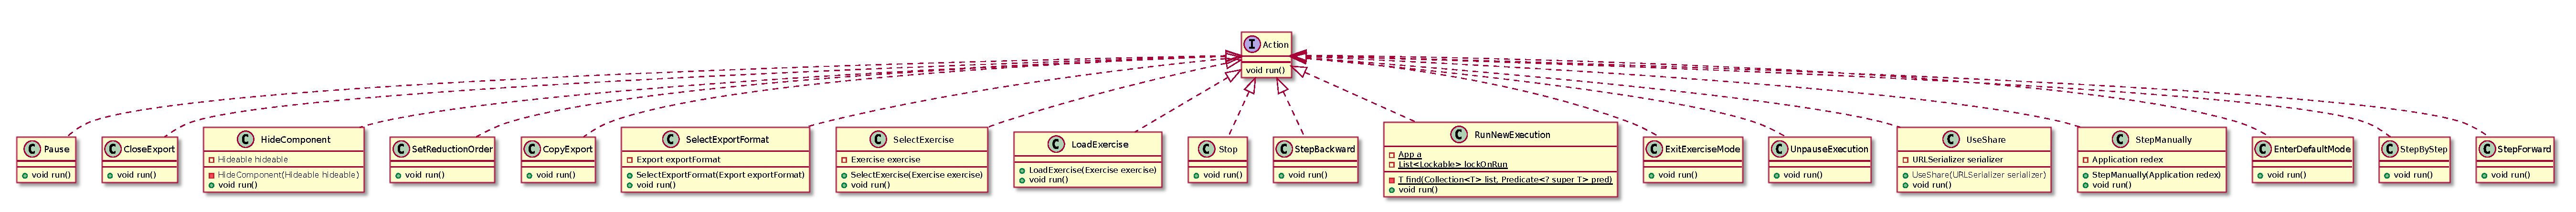
\includegraphics[width=\textwidth]{packageDiagrams/actionPackage}
\end{figure}
